% 若编译失败,且生成 .synctex(busy) 辅助文件,可能有两个原因:
% 1. 需要插入的图片不存在:Ctrl + F 搜索 'figure' 将这些代码注释/删除掉即可
% 2. 路径/文件名含中文或空格:更改路径/文件名即可

% ------------------------------------------------------------- %
% >> ------------------ 文章宏包及相关设置 ------------------ << %
% 设定文章类型与编码格式
\documentclass[UTF8]{report}		

% 本文特殊宏包
\usepackage{siunitx} % 埃米单位

% 本 .tex 专属的宏定义
    \def\V{\ \mathrm{V}}
    \def\mV{\ \mathrm{mV}}
    \def\kV{\ \mathrm{KV}}
    \def\KV{\ \mathrm{KV}}
    \def\MV{\ \mathrm{MV}}
    \def\A{\ \mathrm{A}}
    \def\mA{\ \mathrm{mA}}
    \def\kA{\ \mathrm{KA}}
    \def\KA{\ \mathrm{KA}}
    \def\MA{\ \mathrm{MA}}
    \def\O{\ \Omega}
    \def\mO{\ \Omega}
    \def\kO{\ \mathrm{K}\Omega}
    \def\KO{\ \mathrm{K}\Omega}
    \def\MO{\ \mathrm{M}\Omega}
    \def\Hz{\ \mathrm{Hz}}

% 自定义宏定义
    \def\N{\mathbb{N}}
    \def\F{\mathbb{F}}
    \def\Z{\mathbb{Z}}
    \def\Q{\mathbb{Q}}
    \def\R{\mathbb{R}}
    \def\C{\mathbb{C}}
    \def\T{\mathbb{T}}
    \def\S{\mathbb{S}}
    \def\A{\mathbb{A}}
    \def\I{\mathscr{I}}
    \def\Im{\mathrm{Im\,}}
    \def\Re{\mathrm{Re\,}}
    \def\d{\mathrm{d}}
    \def\p{\partial}

% 导入基本宏包
    \usepackage[UTF8]{ctex}     % 设置文档为中文语言
    \usepackage[colorlinks, linkcolor=blue, anchorcolor=blue, citecolor=blue, urlcolor=blue]{hyperref}  % 宏包:自动生成超链接 (此宏包与标题中的数学环境冲突)
    % \usepackage{hyperref}  % 宏包:自动生成超链接 (此宏包与标题中的数学环境冲突)
    % \hypersetup{
    %     colorlinks=true,    % false:边框链接 ; true:彩色链接
    %     citecolor={blue},    % 文献引用颜色
    %     linkcolor={blue},   % 目录 (我们在目录处单独设置),公式,图表,脚注等内部链接颜色
    %     urlcolor={orange},    % 网页 URL 链接颜色,包括 \href 中的 text
    %     % cyan 浅蓝色 
    %     % magenta 洋红色
    %     % yellow 黄色
    %     % black 黑色
    %     % white 白色
    %     % red 红色
    %     % green 绿色
    %     % blue 蓝色
    %     % gray 灰色
    %     % darkgray 深灰色
    %     % lightgray 浅灰色
    %     % brown 棕色
    %     % lime 石灰色
    %     % olive 橄榄色
    %     % orange 橙色
    %     % pink 粉红色
    %     % purple 紫色
    %     % teal 蓝绿色
    %     % violet 紫罗兰色
    % }

    % \usepackage{docmute}    % 宏包:子文件导入时自动去除导言区,用于主/子文件的写作方式,\include{./51单片机笔记}即可。注:启用此宏包会导致.tex文件capacity受限。
    \usepackage{amsmath}    % 宏包:数学公式
    \usepackage{mathrsfs}   % 宏包:提供更多数学符号
    \usepackage{amssymb}    % 宏包:提供更多数学符号
    \usepackage{pifont}     % 宏包:提供了特殊符号和字体
    \usepackage{extarrows}  % 宏包:更多箭头符号
    \usepackage{multicol}   % 宏包:支持多栏 
    \usepackage{graphicx}   % 宏包:插入图片
    \usepackage{float}      % 宏包:设置图片浮动位置
    %\usepackage{article}    % 宏包:使文本排版更加优美
    \usepackage{tikz}       % 宏包:绘图工具
    %\usepackage{pgfplots}   % 宏包:绘图工具
    \usepackage{enumerate}  % 宏包:列表环境设置
    \usepackage{enumitem}   % 宏包:列表环境设置

% 文章页面margin设置
    \usepackage[a4paper]{geometry}
        \geometry{top=1in}
        \geometry{bottom=1in}
        \geometry{left=0.75in}
        \geometry{right=0.75in}   % 设置上下左右页边距
        \geometry{marginparwidth=1.75cm}    % 设置边注距离(注释、标记等)

% 定义 solution 环境
\usepackage{amsthm}
\newtheorem{solution}{Solution}
        \geometry{bottom=1in}
        \geometry{left=0.75in}
        \geometry{right=0.75in}   % 设置上下左右页边距
        \geometry{marginparwidth=1.75cm}    % 设置边注距离(注释、标记等)

% 配置数学环境
    \usepackage{amsthm} % 宏包:数学环境配置
    % theorem-line 环境自定义
        \newtheoremstyle{MyLineTheoremStyle}% <name>
            {11pt}% <space above>
            {11pt}% <space below>
            {}% <body font> 使用默认正文字体
            {}% <indent amount>
            {\bfseries}% <theorem head font> 设置标题项为加粗
            {:}% <punctuation after theorem head>
            {.5em}% <space after theorem head>
            {\textbf{#1}\thmnumber{#2}\ \ (\,\textbf{#3}\,)}% 设置标题内容顺序
        \theoremstyle{MyLineTheoremStyle} % 应用自定义的定理样式
        \newtheorem{LineTheorem}{Theorem.\,}
    % theorem-block 环境自定义
        \newtheoremstyle{MyBlockTheoremStyle}% <name>
            {11pt}% <space above>
            {11pt}% <space below>
            {}% <body font> 使用默认正文字体
            {}% <indent amount>
            {\bfseries}% <theorem head font> 设置标题项为加粗
            {:\\ \indent}% <punctuation after theorem head>
            {.5em}% <space after theorem head>
            {\textbf{#1}\thmnumber{#2}\ \ (\,\textbf{#3}\,)}% 设置标题内容顺序
        \theoremstyle{MyBlockTheoremStyle} % 应用自定义的定理样式
        \newtheorem{BlockTheorem}[LineTheorem]{Theorem.\,} % 使用 LineTheorem 的计数器
    % definition 环境自定义
        \newtheoremstyle{MySubsubsectionStyle}% <name>
            {11pt}% <space above>
            {11pt}% <space below>
            {}% <body font> 使用默认正文字体
            {}% <indent amount>
            {\bfseries}% <theorem head font> 设置标题项为加粗
           % {:\\ \indent}% <punctuation after theorem head>
            {\\\indent}
            {0pt}% <space after theorem head>
            {\textbf{#3}}% 设置标题内容顺序
        \theoremstyle{MySubsubsectionStyle} % 应用自定义的定理样式
        \newtheorem{definition}{}

%宏包:有色文本框(proof环境)及其设置
    \usepackage[dvipsnames,svgnames]{xcolor}    %设置插入的文本框颜色
    \usepackage[strict]{changepage}     % 提供一个 adjustwidth 环境
    \usepackage{framed}     % 实现方框效果
        \definecolor{graybox_color}{rgb}{0.95,0.95,0.96} % 文本框颜色。修改此行中的 rgb 数值即可改变方框纹颜色,具体颜色的rgb数值可以在网站https://colordrop.io/ 中获得。(截止目前的尝试还没有成功过,感觉单位不一样)(找到喜欢的颜色,点击下方的小眼睛,找到rgb值,复制修改即可)
        \newenvironment{graybox}{%
        \def\FrameCommand{%
        \hspace{1pt}%
        {\color{gray}\small \vrule width 2pt}%
        {\color{graybox_color}\vrule width 4pt}%
        \colorbox{graybox_color}%
        }%
        \MakeFramed{\advance\hsize-\width\FrameRestore}%
        \noindent\hspace{-4.55pt}% disable indenting first paragraph
        \begin{adjustwidth}{}{7pt}%
        \vspace{2pt}\vspace{2pt}%
        }
        {%
        \vspace{2pt}\end{adjustwidth}\endMakeFramed%
        }



% 外源代码插入设置
    % matlab 代码插入设置
    \usepackage{matlab-prettifier}
        \lstset{style=Matlab-editor}    % 继承 matlab 代码高亮 , 此行不能删去
    \usepackage[most]{tcolorbox} % 引入tcolorbox包 
    \usepackage{listings} % 引入listings包
        \tcbuselibrary{listings, skins, breakable}
        \newfontfamily\codefont{Consolas} % 定义需要的 codefont 字体
        \lstdefinestyle{MatlabStyle_inc}{   % 插入代码的样式
            language=Matlab,
            basicstyle=\small\ttfamily\codefont,    % ttfamily 确保等宽 
            breakatwhitespace=false,
            breaklines=true,
            captionpos=b,
            keepspaces=true,
            numbers=left,
            numbersep=15pt,
            showspaces=false,
            showstringspaces=false,
            showtabs=false,
            tabsize=2,
            xleftmargin=15pt,   % 左边距
            %frame=single, % single 为包围式单线框
            frame=shadowbox,    % shadowbox 为带阴影包围式单线框效果
            %escapeinside=``,   % 允许在代码块中使用 LaTeX 命令 (此行无用)
            %frameround=tttt,    % tttt 表示四个角都是圆角
            framextopmargin=0pt,    % 边框上边距
            framexbottommargin=0pt, % 边框下边距
            framexleftmargin=5pt,   % 边框左边距
            framexrightmargin=5pt,  % 边框右边距
            rulesepcolor=\color{red!20!green!20!blue!20}, % 阴影框颜色设置
            %backgroundcolor=\color{blue!10}, % 背景颜色
        }
        \lstdefinestyle{MatlabStyle_src}{   % 插入代码的样式
            language=Matlab,
            basicstyle=\small\ttfamily\codefont,    % ttfamily 确保等宽 
            breakatwhitespace=false,
            breaklines=true,
            captionpos=b,
            keepspaces=true,
            numbers=left,
            numbersep=15pt,
            showspaces=false,
            showstringspaces=false,
            showtabs=false,
            tabsize=2,
        }
        \newtcblisting{matlablisting}{
            %arc=2pt,        % 圆角半径
            % 调整代码在 listing 中的位置以和引入文件时的格式相同
            top=0pt,
            bottom=0pt,
            left=-5pt,
            right=-5pt,
            listing only,   % 此句不能删去
            listing style=MatlabStyle_src,
            breakable,
            colback=white,   % 选一个合适的颜色
            colframe=black!0,   % 感叹号后跟不透明度 (为 0 时完全透明)
        }
        \lstset{
            style=MatlabStyle_inc,
        }



% table 支持
    \usepackage{booktabs}   % 宏包:三线表
    %\usepackage{tabularray} % 宏包:表格排版
    %\usepackage{longtable}  % 宏包:长表格
    %\usepackage[longtable]{multirow} % 宏包:multi 行列


% figure 设置
\usepackage{graphicx}   % 支持 jpg, png, eps, pdf 图片 
\usepackage{float}      % 支持 H 选项
\usepackage{svg}        % 支持 svg 图片
\usepackage{subcaption} % 支持子图
\svgsetup{
        % 指向 inkscape.exe 的路径
       inkscapeexe = C:/aa_MySame/inkscape/bin/inkscape.exe, 
        % 一定程度上修复导入后图片文字溢出几何图形的问题
       inkscapelatex = false                 
   }

% 图表进阶设置
    \usepackage{caption}    % 图注、表注
        \captionsetup[figure]{name=图}  
        \captionsetup[table]{name=表}
        \captionsetup{
            labelfont=bf, % 设置标签为粗体
            textfont=bf,  % 设置文本为粗体
            font=small  
        }
    \usepackage{float}     % 图表位置浮动设置 
        % \floatstyle{plaintop} % 设置表格标题在表格上方
        % \restylefloat{table}  % 应用设置


% 圆圈序号自定义
    \newcommand*\circled[1]{\tikz[baseline=(char.base)]{\node[shape=circle,draw,inner sep=0.8pt, line width = 0.03em] (char) {\small \bfseries #1};}}   % TikZ solution


% 列表设置
    \usepackage{enumitem}   % 宏包:列表环境设置
        \setlist[enumerate]{
            label=\bfseries(\arabic*) ,   % 设置序号样式为加粗的 (1) (2) (3)
            ref=\arabic*, % 如果需要引用列表项,这将决定引用格式(这里仍然使用数字)
            itemsep=0pt, parsep=0pt, topsep=0pt, partopsep=0pt, leftmargin=3.5em} 
        \setlist[itemize]{itemsep=0pt, parsep=0pt, topsep=0pt, partopsep=0pt, leftmargin=3.5em}
        \newlist{circledenum}{enumerate}{1} % 创建一个新的枚举环境  
        \setlist[circledenum,1]{  
            label=\protect\circled{\arabic*}, % 使用 \arabic* 来获取当前枚举计数器的值,并用 \circled 包装它  
            ref=\arabic*, % 如果需要引用列表项,这将决定引用格式(这里仍然使用数字)
            itemsep=0pt, parsep=0pt, topsep=0pt, partopsep=0pt, leftmargin=3.5em
        }  

% 文章默认字体设置
    \usepackage{fontspec}   % 宏包:字体设置
        \setmainfont{STKaiti}    % 设置中文字体为宋体字体
        \setCJKmainfont[AutoFakeBold=3]{STKaiti} % 设置加粗字体为 STKaiti 族,AutoFakeBold 可以调整字体粗细
        \setmainfont{Times New Roman} % 设置英文字体为Times New Roman


% 其它设置
    % 脚注设置
    \renewcommand\thefootnote{\ding{\numexpr171+\value{footnote}}}
    % 参考文献引用设置
        \bibliographystyle{unsrt}   % 设置参考文献引用格式为unsrt
        \newcommand{\upcite}[1]{\textsuperscript{\cite{#1}}}     % 自定义上角标式引用
    % 文章序言设置
        \newcommand{\cnabstractname}{序言}
        \newenvironment{cnabstract}{%
            \par\Large
            \noindent\mbox{}\hfill{\bfseries \cnabstractname}\hfill\mbox{}\par
            \vskip 2.5ex
            }{\par\vskip 2.5ex}


% 各级标题自定义设置
    \usepackage{titlesec}   
    % chapter
        \titleformat{\chapter}[hang]{\normalfont\Large\bfseries\centering}{题目}{10pt}{}
        \titlespacing*{\chapter}{0pt}{-30pt}{10pt} % 控制上方空白的大小
    % section
        \titleformat{\section}[hang]{\normalfont\large\bfseries}{\thesection}{8pt}{}
    % subsection
        %\titleformat{\subsubsection}[hang]{\normalfont\bfseries}{}{8pt}{}
    % subsubsection
        %\titleformat{\subsubsection}[hang]{\normalfont\bfseries}{}{8pt}{}

% 见到的一个有意思的对于公式中符号的彩色解释的环境
        \usepackage[dvipsnames]{xcolor}
        \usepackage{tikz}
        \usetikzlibrary{backgrounds}
        \usetikzlibrary{arrows,shapes}
        \usetikzlibrary{tikzmark}
        \usetikzlibrary{calc}
        
        \usepackage{amsmath}
        \usepackage{amsthm}
        \usepackage{amssymb}
        \usepackage{mathtools, nccmath}
        \usepackage{wrapfig}
        \usepackage{comment}
        
        % To generate dummy text
        \usepackage{blindtext}
        
        
        %color
        %\usepackage[dvipsnames]{xcolor}
        % \usepackage{xcolor}
        
        
        %\usepackage[pdftex]{graphicx}
        \usepackage{graphicx}
        % declare the path(s) for graphic files
        %\graphicspath{{../Figures/}}
        
        % extensions so you won't have to specify these with
        % every instance of \includegraphics
        % \DeclareGraphicsExtensions{.pdf,.jpeg,.png}
        
        % for custom commands
        \usepackage{xspace}
        
        % table alignment
        \usepackage{array}
        \usepackage{ragged2e}
        \newcolumntype{P}[1]{>{\RaggedRight\hspace{0pt}}p{#1}}
        \newcolumntype{X}[1]{>{\RaggedRight\hspace*{0pt}}p{#1}}
        
        % color box
        \usepackage{tcolorbox}
        
        
        % for tikz
        \usepackage{tikz}
        %\usetikzlibrary{trees}
        \usetikzlibrary{arrows,shapes,positioning,shadows,trees,mindmap}
        \usetikzlibrary{graphs} % <-- Added for \graph syntax
        % \usepackage{forest}
        \usepackage[edges]{forest}
        \usetikzlibrary{arrows.meta}
        \colorlet{linecol}{black!75}
        \usepackage{xkcdcolors} % xkcd colors
        
        
        % for colorful equation
        \usepackage{tikz}
        \usetikzlibrary{backgrounds}
        \usetikzlibrary{arrows,shapes}
        \usetikzlibrary{tikzmark}
        \usetikzlibrary{calc}
        % Commands for Highlighting text -- non tikz method
        \newcommand{\highlight}[2]{\colorbox{#1!17}{$\displaystyle #2$}}
        %\newcommand{\highlight}[2]{\colorbox{#1!17}{$#2$}}
        \newcommand{\highlightdark}[2]{\colorbox{#1!47}{$\displaystyle #2$}}
        
        % my custom colors for shading
        \colorlet{mhpurple}{Plum!80}
        
        
        % Commands for Highlighting text -- non tikz method
        \renewcommand{\highlight}[2]{\colorbox{#1!17}{#2}}
        \renewcommand{\highlightdark}[2]{\colorbox{#1!47}{#2}}
        
        % Some math definitions
        \newcommand{\lap}{\mathrm{Lap}}
        \newcommand{\pr}{\mathrm{Pr}}
        
        \newcommand{\Tset}{\mathcal{T}}
        \newcommand{\Dset}{\mathcal{D}}
        \newcommand{\Rbound}{\widetilde{\mathcal{R}}}

% >> ------------------ 文章宏包及相关设置 ------------------ << %
% ------------------------------------------------------------- %



% ----------------------------------------------------------- %
% >> --------------------- 文章信息区 --------------------- << %
% 页眉页脚设置

\usepackage{fancyhdr}   %宏包:页眉页脚设置
    \pagestyle{fancy}
    \fancyhf{}
    \cfoot{\thepage}
    \renewcommand\headrulewidth{1pt}
    \renewcommand\footrulewidth{0pt}
    \rhead{数据结构与算法期末复习,\ 尹超,\ 2023K8009926003}
    \lhead{Homework}


%文档信息设置
\title{数据结构与算法期末复习\\ Homework}
\author{尹超\\ \footnotesize 中国科学院大学,北京 100049\\ Carter Yin \\ \footnotesize University of Chinese Academy of Sciences, Beijing 100049, China}
\date{\footnotesize 2024.8 -- 2025.1}
% >> --------------------- 文章信息区 --------------------- << %
% ----------------------------------------------------------- %     


% 开始编辑文章

% 定义 tikz 样式 splaynode 和 highlight
\tikzset{
  splaynode/.style={draw, circle, minimum size=7mm, inner sep=0pt},
  highlight/.style={draw, circle, minimum size=7mm, inner sep=0pt, fill=yellow!30}
}

\begin{document}
\zihao{5}           % 设置全文字号大小

% --------------------------------------------------------------- %
% >> --------------------- 封面序言与目录 --------------------- << %
% 封面
    \maketitle\newpage  
    \pagenumbering{Roman} % 页码为大写罗马数字
    \thispagestyle{fancy}   % 显示页码、页眉等

% 序言
    \begin{cnabstract}\normalsize 
        本文为笔者数据结构与算法的期末复习笔记。\par
        望老师批评指正。
    \end{cnabstract}
    \addcontentsline{toc}{chapter}{序言} % 手动添加为目录

% % 不换页目录
%     \setcounter{tocdepth}{0}
%     \noindent\rule{\textwidth}{0.1em}   % 分割线
%     \noindent\begin{minipage}{\textwidth}\centering 
%         \vspace{1cm}
%         \tableofcontents\thispagestyle{fancy}   % 显示页码、页眉等   
%     \end{minipage}  
%     \addcontentsline{toc}{chapter}{目录} % 手动添加为目录

% 目录
\setcounter{tocdepth}{4}                % 目录深度(为1时显示到section)
\tableofcontents                        % 目录页
\addcontentsline{toc}{chapter}{目录}    % 手动添加此页为目录
\thispagestyle{fancy}                   % 显示页码、页眉等 

% 收尾工作
    \newpage    
    \pagenumbering{arabic} 

% >> --------------------- 封面序言与目录 --------------------- << %
% --------------------------------------------------------------- %

\chapter{第九章 图}

\section*{151}
\begin{graybox}
任何两个顶点间都有一条(无向)边的图称
为完全图,包含n个顶点的完全图用Kn表示。下列
哪个图一定不是平面图?
A. K2
B. K3
C. K4
D. K5
\end{graybox}

\begin{solution}
正确答案是 D。

\textbf{详细分析:}

一个图是\textbf{平面图}(Planar Graph),如果它可以在一个平面上被画出来,且没有任何两条边相互交叉(除了在顶点处相交)。

\begin{itemize}
    \item \textbf{A. K2}: 包含2个顶点和1条边。它是一条线段,显然是平面图。
    \begin{center}
    \begin{tikzpicture}
      \graph { 1 -- 2 };
    \end{tikzpicture}
    \end{center}

    \item \textbf{B. K3}: 包含3个顶点和3条边。它是一个三角形,显然是平面图。
    \begin{center}
    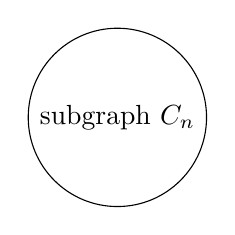
\begin{tikzpicture}
      \graph [nodes={circle, draw}, n=3, clockwise] { subgraph $C_n$ };
    \end{tikzpicture}
    \end{center}

    \item \textbf{C. K4}: 包含4个顶点和6条边。它可以被画成一个带两条对角线的正方形。虽然对角线会交叉,但我们可以重新绘制它,使得边不交叉(例如,将一个顶点放在其他三个顶点构成的三角形内部)。因此,K4是平面图。
    \begin{center}
    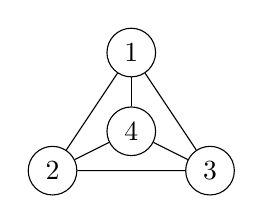
\begin{tikzpicture}
      \node[circle, draw] (1) at (0,1) {1};
      \node[circle, draw] (2) at (-1,-0.5) {2};
      \node[circle, draw] (3) at (1,-0.5) {3};
      \node[circle, draw] (4) at (0,0) {4};
      \draw (1)--(2)--(3)--(1);
      \draw (4)--(1);
      \draw (4)--(2);
      \draw (4)--(3);
    \end{tikzpicture}
    \end{center}

    \item \textbf{D. K5}: 包含5个顶点和 $C(5,2) = 10$ 条边。根据图论中的一个基本结论(库拉托夫斯基定理),\textbf{K5是典型的非平面图}。无论如何绘制,它的边都必然会发生交叉。

    我们可以用欧拉公式的推论来证明这一点:对于任何一个顶点数 $v \ge 3$ 的连通平面图,其边数 $e$ 和顶点数 $v$ 必须满足不等式 $e \le 3v - 6$。
    \begin{itemize}
        \item 对于K5,我们有 $v=5$,$e=10$。
        \item 将这些值代入不等式:$10 \le 3(5) - 6$。
        \item 计算结果为:$10 \le 15 - 6$,即 $10 \le 9$。
        \item 这个不等式显然是\textbf{不成立}的。
    \end{itemize}
    因为K5不满足平面图所必须满足的条件,所以K5一定不是平面图。
\end{itemize}
\end{solution}


\section*{152}
\begin{graybox}
在包含n个顶点的用邻接矩阵实现的图
中,顶点v有m个邻居,遍历所有m个邻居的时
间复杂度为:
A. O(1)
B. O(m)
C. O(n)
D. O(mn)
\end{graybox}

\begin{solution}
正确答案是 C。

\textbf{详细分析:}

\begin{enumerate}
    \item \textbf{邻接矩阵的结构:}
    一个包含n个顶点的图的邻接矩阵是一个 $n \times n$ 的二维数组,我们称之为 `Adj`。如果顶点 `i` 和顶点 `j` 之间有边,则 `Adj[i][j]` 为1(或权重),否则为0。

    \item \textbf{如何查找邻居:}
    要找到顶点 `v` 的所有邻居,我们必须检查邻接矩阵中对应于 `v` 的那\textbf{一整行},即 `Adj[v][0], Adj[v][1], ..., Adj[v][n-1]`。

    \item \textbf{时间复杂度分析:}
    \begin{itemize}
        \item 这一行总共有 `n` 个元素,对应图中所有的 `n` 个顶点。
        \item 我们需要遍历这一行中的所有 `n` 个元素,来判断哪些位置的值为1(表示是邻居)。
        \item 无论顶点 `v` 有多少个实际的邻居(即 `m` 的值是多少),这个遍历过程都必须检查 `n` 次。
        \item 因此,遍历顶点 `v` 所有邻居的时间复杂度取决于顶点的总数 `n`,而不是邻居的数量 `m`。
    \end{itemize}

    \item \textbf{与其他选项的对比:}
    \begin{itemize}
        \item B. O(m): 这个是使用\textbf{邻接表}实现图时,遍历邻居的时间复杂度。因为邻接表只存储了实际存在的边。
        \item A. O(1) 和 D. O(mn): 均不符合邻接矩阵的遍历特性。
    \end{itemize}
\end{enumerate}

\textbf{结论:}
在用邻接矩阵表示的图中,查找一个特定顶点的所有邻居,需要扫描该顶点对应的完整一行,其时间复杂度为 $O(n)$。
\end{solution}


\section*{153}
\begin{graybox}
图G包含n个顶点(n>0),用邻接矩阵实现。
在其中加入一个新的顶点后邻接矩阵增加了多少项?
A. n+1
B. 2n
C. 2n-1
D. 2n+1
\end{graybox}

\begin{solution}
正确答案是 D。

\textbf{详细分析:}

\begin{enumerate}
    \item \textbf{初始状态:}
    \begin{itemize}
        \item 图G有 `n` 个顶点。
        \item 其邻接矩阵是一个 `n x n` 的方阵。
        \item 矩阵中的总项数(元素个数)为 $n \times n = n^2$。
    \end{itemize}

    \item \textbf{加入新顶点后的状态:}
    \begin{itemize}
        \item 图G现在有 `n + 1` 个顶点。
        \item 其邻接矩阵变为一个 `(n+1) x (n+1)` 的方阵。
        \item 新矩阵中的总项数为 $(n+1) \times (n+1) = (n+1)^2$。
    \end{itemize}

    \item \textbf{计算增加的项数:}
    增加的项数等于新矩阵的总项数减去旧矩阵的总项数。
    \begin{itemize}
        \item 增加的项数 = $(n+1)^2 - n^2$
        \item 展开 $(n+1)^2$:$n^2 + 2n + 1$
        \item 计算差值:$(n^2 + 2n + 1) - n^2 = 2n + 1$
    \end{itemize}
\end{enumerate}

\textbf{直观理解:}
当从一个 $n \times n$ 矩阵变为一个 $(n+1) \times (n+1)$ 矩阵时,相当于增加了一行和一列。
\begin{itemize}
    \item 增加的行有 `n+1` 个元素。
    \item 增加的列有 `n+1` 个元素。
    \item 其中,新行和新列的交叉点 `A[n+1][n+1]` 被计算了两次,所以要减去1。
    \item 总增加量 = (新行的元素数) + (新列的元素数) - (重复计算的1个元素) = $(n+1) + (n+1) - 1 = 2n + 2 - 1 = 2n + 1$。
\end{itemize}

因此,邻接矩阵增加了 `2n + 1` 项。
\end{solution}


\section*{154}
\begin{graybox}
图的广度优先搜索访问各顶点的模式类
似于二叉树的:
A. 先序遍历
B. 中序遍历
C. 后序遍历
D. 层次遍历
\end{graybox}

\begin{solution}
正确答案是 D。

\textbf{详细分析:}

\begin{enumerate}
    \item \textbf{图的广度优先搜索 (BFS - Breadth-First Search):}
    \begin{itemize}
        \item BFS从一个起始顶点开始,首先访问所有与起始顶点直接相邻的顶点。
        \item 然后,再逐一访问与这些邻接点相邻的、尚未被访问过的顶点。
        \item 这个过程一层一层地向外扩展,就像水波纹一样。
        \item BFS通常使用一个队列(Queue)数据结构来实现,以保证“先发现的顶点,其邻居也先被探索”的顺序。
    \end{itemize}

    \item \textbf{二叉树的遍历方式:}
    \begin{itemize}
        \item \textbf{A, B, C (先序、中序、后序遍历):} 这三种都是\textbf{深度优先遍历 (DFS - Depth-First Search)}的特例。它们会沿着一条路径尽可能深地访问下去,直到末端,然后再回溯。这与BFS的逐层扩展模式完全不同。
        \item \textbf{D. 层次遍历 (Level-Order Traversal):} 层次遍历从树的根节点开始,按照从上到下、从左到右的顺序,逐层访问树中的所有节点。它也是使用队列来实现的。
    \end{itemize}
\end{enumerate}

\textbf{结论:}
图的广度优先搜索(BFS)和二叉树的层次遍历在思想和实现上是完全一致的。它们都是逐层地访问节点,并且都依赖于队列来管理待访问的节点顺序。因此,BFS的访问模式类似于二叉树的层次遍历。
\end{solution}


\section*{155}
\begin{graybox}
以顶点s为起点对以上无向图进行BFS,同一
顶点的邻居之间以a~z为顺序,顶点c刚出队时队列
中顶点从队头到队尾为:
\begin{center}
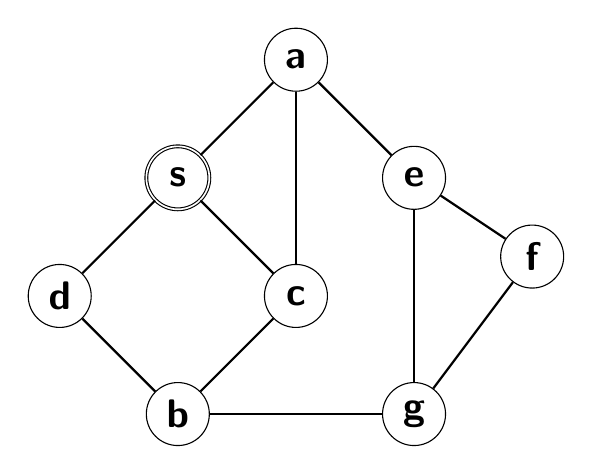
\begin{tikzpicture}[
    main_node/.style={circle, draw, font=\sffamily\Large\bfseries, minimum size=8mm},
    start_node/.style={circle, double, draw, font=\sffamily\Large\bfseries, minimum size=8mm}
]

% 定義節點位置 (Define node positions)
\node[main_node] (a) at (0, 3) {a};
\node[start_node] (s) at (-1.5, 1.5) {s};
\node[main_node] (e) at (1.5, 1.5) {e};
\node[main_node] (d) at (-3, 0) {d};
\node[main_node] (c) at (0, 0) {c};
\node[main_node] (f) at (3, 0.5) {f};
\node[main_node] (b) at (-1.5, -1.5) {b};
\node[main_node] (g) at (1.5, -1.5) {g};

% 連接節點 (Connect the nodes)
\path[draw, thick]
    (a) edge (s)
    (a) edge (c)
    (a) edge (e)
    (s) edge (d)
    (s) edge (c)
    (d) edge (b)
    (c) edge (b)
    (b) edge (g)
    (e) edge (f)
    (e) edge (g)
    (f) edge (g);

\end{tikzpicture}
\end{center}
A. d, e\\
B. e, d\\
C. d, a\\
D. a, d
\end{graybox}

\begin{solution}
正确答案是 A。

\textbf{详细分析:}

我们来逐步模拟广度优先搜索(BFS)的过程。BFS使用一个队列来管理待访问的顶点。

\begin{enumerate}
    \item \textbf{初始状态:}
    \begin{itemize}
        \item 起点为 \textbf{s}。将 \textbf{s} 入队。
        \item 队列:`[s]`
    \end{itemize}

    \item \textbf{第一次出队:}
    \begin{itemize}
        \item 顶点 \textbf{s} 出队。
        \item 查找 \textbf{s} 的所有邻居:a, c, d。
        \item 按字母顺序排序:a, c, d。
        \item 将 a, c, d 依次入队。
        \item 队列:`[a, c, d]`
    \end{itemize}

    \item \textbf{第二次出队:}
    \begin{itemize}
        \item 顶点 \textbf{a} 出队。
        \item 查找 \textbf{a} 的所有邻居:c, e, s。
        \item 按字母顺序排序:c, e, s。
        \item 检查邻居是否已被访问(即是否已在队列中或已出队):
            \begin{itemize}
                \item c: 已在队列中,跳过。
                \item e: 未被访问,将 \textbf{e} 入队。
                \item s: 已被访问,跳过。
            \end{itemize}
        \item 队列:`[c, d, e]`
    \end{itemize}

    \item \textbf{第三次出队:}
    \begin{itemize}
        \item 顶点 \textbf{c} 出队。
        \item 此时,我们观察队列的状态。
        \item 队列中剩下的顶点,从队头到队尾依次是:\textbf{d, e}。
    \end{itemize}
\end{enumerate}

因此,当顶点c刚出队时,队列中的顶点为 d, e。
\end{solution}


\section*{156}
\begin{graybox}
对于用邻接表实现的包含n个顶点e条边
的图,BFS的时间复杂度为:\\
A. O(n)\\
B. O($n^2$)\\
C. O(n+e)\\
D. O($n^2$+e)\\
\end{graybox}

\begin{solution}
正确答案是 C。

\textbf{详细分析:}

广度优先搜索(BFS)在邻接表实现的图上的时间复杂度可以从两个主要部分来分析:

\begin{enumerate}
    \item \textbf{顶点操作:}
    \begin{itemize}
        \item BFS需要访问图中的每一个顶点。
        \item 每个顶点都会被入队(enqueue)一次和出队(dequeue)一次。
        \item 假设有 `n` 个顶点,这部分操作的总时间复杂度是 $O(n)$。
    \end{itemize}

    \item \textbf{边操作:}
    \begin{itemize}
        \item 当一个顶点 `v` 从队列中出队时,BFS会遍历 `v` 的邻接表,以找到所有与它相邻的顶点。
        \item 在整个BFS的执行过程中,每个顶点的邻接表都会被完整地遍历一次。
        \item 在邻接表表示法中,所有邻接表的长度之和等于图的总边数 `e`(对于有向图)或 `2e`(对于无向图)。无论哪种情况,这部分操作的总时间复杂度都与边的数量成正比,即 $O(e)$。
    \end{itemize}
\end{enumerate}

\textbf{结论:}
将顶点操作和边操作的时间复杂度相加,得到BFS在邻接表上实现的总时间复杂度为 $O(n) + O(e) = O(n+e)$。

(注:如果图是用邻接矩阵实现的,由于查找每个顶点的邻居都需要扫描一行,总时间复杂度会是 $O(n^2)$。)
\end{solution}



\section*{157}
\begin{graybox}
以A为起点对以下无向图进行DFS,同一顶点
的邻居以a~z为序,各顶点被访问的顺序为:
\begin{center}
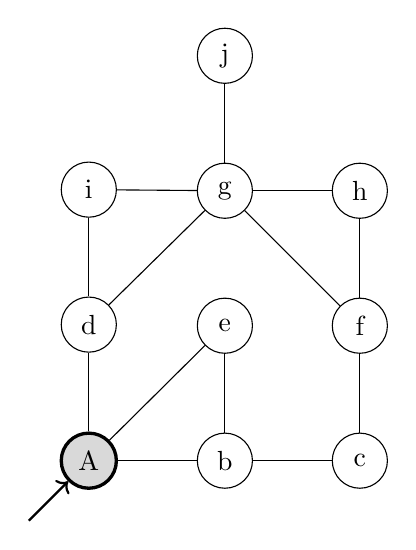
\begin{tikzpicture}[
    node distance=1cm and 1cm, % Horizontal and vertical distance between nodes
    every node/.style={circle, draw, minimum size=0.7cm}, % Style for all nodes
    highlight node/.style={circle, draw, fill=gray!30, minimum size=0.7cm, very thick} % Style for highlighted node
]

    % Define nodes
    \node (A) [highlight node] {A};
    \node (b) [right=of A] {b};
    \node (c) [right=of b] {c};
    \node (d) [above=of A] {d};
    \node (e) [above=of b] {e};
    \node (f) [above=of c] {f};
    \node (i) [above=of d] {i};
    \node (g) [above=of e] {g};
    \node (h) [above=of f] {h};
    \node (j) [above=of g] {j};

    % Draw edges
    \draw (A) -- (b);
    \draw (b) -- (c);
    \draw (A) -- (d);
    \draw (b) -- (e);
    \draw (c) -- (f);
    \draw (d) -- (i);
    \draw (d) -- (g);
    \draw (e) -- (A); % This edge is diagonal in the image
    \draw (f) -- (g);
    \draw (f) -- (h);
    \draw (i) -- (g);
    \draw (g) -- (h);
    \draw (g) -- (j);
    
    % Add the small arrow pointing to A
    \draw[->, thick] ([xshift=-0.5cm, yshift=-0.5cm]A.south west) -- (A.south west);

\end{tikzpicture}
\end{center}
A. a, e, b, c, f, g, h, j, i, d\\
B. a, b, c, f, g, d, i, h, j, e\\
C. a, b, e, c, f, h, g, i, d, j\\
D. a, e, b, c, f, h, g, i, d, j
\end{graybox}

\begin{solution}
正确答案是 B。

\textbf{详细分析:}

我们使用递归(或栈)来模拟深度优先搜索(DFS)的过程。
首先,列出每个顶点的邻居,并按字母顺序排序:
\begin{itemize}
    \item \textbf{A}: b, d, e
    \item \textbf{b}: A, c, e
    \item \textbf{c}: b, f
    \item \textbf{d}: A, g, i
    \item \textbf{e}: A, b
    \item \textbf{f}: c, g, h
    \item \textbf{g}: d, f, h, i, j
    \item \textbf{h}: f, g
    \item \textbf{i}: d, g
    \item \textbf{j}: g
\end{itemize}

\textbf{DFS 步骤:}
\begin{enumerate}
    \item \textbf{访问 A}。邻居是 b, d, e。选择第一个未访问的 \textbf{b}。
    \item \textbf{访问 b}。邻居是 A, c, e。A已访问,选择第一个未访问的 \textbf{c}。
    \item \textbf{访问 c}。邻居是 b, f。b已访问,选择第一个未访问的 \textbf{f}。
    \item \textbf{访问 f}。邻居是 c, g, h。c已访问,选择第一个未访问的 \textbf{g}。
    \item \textbf{访问 g}。邻居是 d, f, h, i, j。f已访问,选择第一个未访问的 \textbf{d}。
    \item \textbf{访问 d}。邻居是 A, g, i。A, g已访问,选择第一个未访问的 \textbf{i}。
    \item \textbf{访问 i}。邻居是 d, g。d, g都已访问。回溯到 d。
    \item 从 d 回溯到 g。
    \item 在 g,邻居是 d, f, h, i, j。d, f, i已访问,选择下一个未访问的 \textbf{h}。
    \item \textbf{访问 h}。邻居是 f, g。f, g都已访问。回溯到 g。
    \item 在 g,邻居是 d, f, h, i, j。d, f, h, i已访问,选择下一个未访问的 \textbf{j}。
    \item \textbf{访问 j}。邻居是 g。g已访问。回溯到 g。
    \item 从 g 回溯到 f,再到 c,再到 b。
    \item 在 b,邻居是 A, c, e。A, c已访问,选择下一个未访问的 \textbf{e}。
    \item \textbf{访问 e}。邻居是 A, b。A, b都已访问。回溯到 b。
    \item 从 b 回溯到 A。
    \item 在 A,所有邻居 b, d, e 都已被访问。搜索结束。
\end{enumerate}

\textbf{最终访问顺序为:}
A $\rightarrow$ b $\rightarrow$ c $\rightarrow$ f $\rightarrow$ g $\rightarrow$ d $\rightarrow$ i $\rightarrow$ h $\rightarrow$ j $\rightarrow$ e
\end{solution}


\section*{158}
\begin{graybox}
u和v为图中两个顶点,对图进行DFS后,
dTime(u) < dTime(v) < fTime(v) <
fTime(u),则u和v在DFS森林中的关系是:
A. 属于不同的连通分量
B. u 为 v 的祖先
C. v 为 u 的祖先
D. 互为兄弟
\end{graybox}

\begin{solution}
正确答案是 B。

\textbf{详细分析:}

在图的深度优先搜索(DFS)中,每个顶点 `v` 都有两个时间戳:
\begin{itemize}
    \item \textbf{dTime(v)}: 发现时间(Discovery Time),即 `v` 第一次被访问的时间。
    \item \textbf{fTime(v)}: 完成时间(Finishing Time),即 `v` 的邻接表被完全扫描完毕,搜索从 `v` 回溯的时间。
\end{itemize}

这些时间戳之间存在一个重要的性质,称为\textbf{“括号引理”(Parenthesis Theorem)}。它描述了任意两个顶点 `u` 和 `v` 的时间戳区间 `[dTime, fTime]` 的关系:

\begin{enumerate}
    \item \textbf{区间不相交:} `dTime(u) < fTime(u) < dTime(v) < fTime(v)` (或u,v交换)。这表示 `u` 和 `v` 在DFS森林中没有祖先-后代关系。它们可能在不同的DFS树中,也可能在同一棵树但属于不同的分支。
    \item \textbf{区间包含:} `dTime(u) < dTime(v) < fTime(v) < fTime(u)`。这表示 `v` 的访问过程完全包含在 `u` 的访问过程中。
\end{enumerate}

我们来分析题目给出的条件:`dTime(u) < dTime(v) < fTime(v) < fTime(u)`。

\begin{itemize}
    \item `dTime(u) < dTime(v)` 意味着 `u` 比 `v` 先被发现。
    \item `fTime(v) < fTime(u)` 意味着 `v` 比 `u` 先完成。
\end{itemize}

这整个过程可以这样理解:
\begin{enumerate}
    \item DFS开始,发现了 `u`。
    \item 在探索 `u` 的后代时,发现了 `v`。
    \item DFS继续探索 `v` 的所有后代,并完成了对 `v` 的访问。
    \item DFS回溯,最终完成了对 `u` 的访问。
\end{enumerate}

这种时间戳的嵌套关系,恰好说明了 `v` 是在 `u` 的DFS子树中被发现和完成的。因此,在DFS森林中,\textbf{u 是 v 的祖先}。

\textbf{其他选项分析:}
\begin{itemize}
    \item A. 属于不同的连通分量:时间区间会不相交。
    \item C. v 为 u 的祖先:时间关系应为 `dTime(v) < dTime(u) < fTime(u) < fTime(v)`。
    \item D. 互为兄弟:时间区间会不相交,例如 `dTime(u) < fTime(u) < dTime(v) < fTime(v)`。
\end{itemize}
\end{solution}


\section*{159}
\begin{graybox}
对同一个无向图分别运行广度优先算法和深
度优先算法,得到的树边数量:
A. 广度优先的树边更
B. 深度优先的树边更多
C. 两种算法得到的树边一样多
D. 数量关系不确定
\end{graybox}

\begin{solution}
正确答案是 C。

\textbf{详细分析:}

\begin{enumerate}
    \item \textbf{遍历与生成树:}
    无论是广度优先搜索(BFS)还是深度优先搜索(DFS),当它们在一个图上运行时,都会将图的边分为两类:树边(Tree Edge)和非树边。树边是那些在遍历过程中连接到一个未访问顶点的边。所有树边集合起来,会构成一个\textbf{生成树}(Spanning Tree)或\textbf{生成森林}(Spanning Forest)。

    \item \textbf{生成树的性质:}
    \begin{itemize}
        \item 对于一个有 `n` 个顶点的\textbf{连通图},其任何一个生成树都恰好包含 `n-1` 条边。这是连接 `n` 个顶点而又不形成环路所需的最少边数。
        \item 对于一个有 `n` 个顶点和 `k` 个连通分量的\textbf{非连通图},其生成森林由 `k` 棵生成树组成,总边数为 `n-k`。
    \end{itemize}

    \item \textbf{比较BFS和DFS:}
    \begin{itemize}
        \item 对一个连通图运行BFS,会访问所有 `n` 个顶点,并产生一个包含 `n-1` 条树边的BFS树。
        \item 对同一个连通图运行DFS,同样会访问所有 `n` 个顶点,并产生一个包含 `n-1` 条树边的DFS树。
        \item 即使图不连通,两个算法也都会访问所有 `n` 个顶点,并为 `k` 个连通分量分别生成树,总边数都是 `n-k`。
    \end{itemize}
\end{enumerate}

\textbf{结论:}
虽然BFS和DFS生成的生成树(或森林)的\textbf{结构}(形状)通常是不同的(BFS树通常更“矮胖”,DFS树通常更“瘦高”),但它们包含的\textbf{树边数量}是完全相同的。这个数量只取决于图本身的顶点数和连通分量数,与所使用的遍历算法无关。
\end{solution}

\section*{160}
\begin{graybox}
对图进行DFS,以下哪种情况意味着该
图包含环路
A. 有TREE边
B. 有BACKWARD边
C. 有FORWARD边
D. 有CROSS边
\end{graybox}

\begin{solution}
正确答案是 B。

\textbf{详细分析:}

在深度优先搜索(DFS)过程中,图中的边可以根据其连接的顶点的状态(发现时间、完成时间)分为四类:

\begin{enumerate}
    \item \textbf{树边 (TREE edge):} 在DFS森林中连接父子节点的边。这是第一次发现一个新顶点时经过的边。树边本身不构成环路。

    \item \textbf{后向边 (BACKWARD edge):} 连接一个顶点 `u` 到其在DFS树中的一个\textbf{祖先} `v` 的边。当DFS从顶点 `u` 探索到其邻居 `v`,而 `v` 已经被访问过且尚未完成(即 `v` 是 `u` 的祖先,仍在当前的递归调用栈中)时,就发现了一条后向边。这条后向边 `(u, v)` 与DFS树中从 `v` 到 `u` 的路径共同构成了一个\textbf{环路}。

    \item \textbf{前向边 (FORWARD edge):} 连接一个顶点 `u` 到其在DFS树中的一个\textbf{后代} `v` 的边(非树边)。

    \item \textbf{横跨边 (CROSS edge):} 连接两个没有祖先-后代关系的顶点的边,它们可能在DFS森林的不同分支或不同的树中。
\end{enumerate}

\textbf{结论:}
\begin{itemize}
    \item A. TREE边是构成DFS生成树(森林)的基本骨架,本身是无环的。
    \item \textbf{B. BACKWARD边是存在环路的决定性标志。} 发现一条后向边就意味着找到了一个环。
    \item C. FORWARD边和 D. CROSS边(主要在有向图中)并不指向当前路径上的祖先节点,因此它们本身不构成环路。
\end{itemize}

因此,在DFS中,判断一个图是否包含环路的标准方法就是检查是否存在后向边。
\end{solution}


\section*{161}
\begin{graybox}
在含20个顶点的简单无向图中,边的数量最
多为:\underline{\hspace{2cm}}
此时度最小的顶点的度为:\underline{\hspace{2cm}}
\end{graybox}

\begin{solution}
\textbf{详细分析:}

\subsection*{第一部分:边的数量最多为多少?}
\begin{enumerate}
    \item 一个“简单无向图”是指图中没有自环(一个顶点到自身的边)也没有重边(两个顶点之间有多于一条边)。
    \item 当一个简单无向图的边数最多时,它是一个\textbf{完全图}(Complete Graph),记作 $K_n$。在完全图中,任意两个不同的顶点之间都恰好有一条边。
    \item 对于一个包含 $n$ 个顶点的图,边的数量就是从这 $n$ 个顶点中选取2个顶点进行组合的数量。
    \item 计算公式为:$C(n, 2) = \frac{n(n-1)}{2}$。
    \item 在本题中,$n=20$,所以边的最大数量为:
    $C(20, 2) = \frac{20 \times (20-1)}{2} = \frac{20 \times 19}{2} = 10 \times 19 = 190$。
\end{enumerate}

\subsection*{第二部分:此时度最小的顶点的度为多少?}
\begin{enumerate}
    \item “此时”指的是在边数最多的情况下,即在完全图 $K_{20}$ 中。
    \item 在一个完全图 $K_n$ 中,每个顶点都与其他所有 $n-1$ 个顶点相连。
    \item 因此,每个顶点的度(degree)都是 $n-1$。
    \item 在本题中,$n=20$,所以 $K_{20}$ 中每个顶点的度都是 $20 - 1 = 19$。
    \item 因为所有顶点的度都是19,所以度最小的顶点的度也是19。
\end{enumerate}

\hrulefill

在含20个顶点的简单无向图中,边的数量最
多为:\underline{\hspace{2cm}\textbf{190}\hspace{2cm}}
此时度最小的顶点的度为:\underline{\hspace{2cm}\textbf{19}\hspace{2cm}}
\end{solution}

\section*{162}
\begin{graybox}
某宴会一共有7个人参加,与会者之间
进行了亲切的握手。已知他们中的每个人进行
握手的次数分别为:
3, 1, 2, 2, 3, 1, 2
请问宴会上总共发生了多少次握手?
\underline{\hspace{2cm}}
\end{graybox}

\begin{solution}
\textbf{详细分析:}

这个问题可以利用图论中的\textbf{握手引理(Handshaking Lemma)}或\textbf{度数总和公式}来解决。

\begin{enumerate}
    \item \textbf{建立图模型:}
    \begin{itemize}
        \item 我们可以将每个参加宴会的人看作图中的一个\textbf{顶点}(Vertex)。
        \item 两个人之间的一次握手可以看作连接对应顶点的\textbf{边}(Edge)。
        \item 每个人握手的次数就是对应顶点的\textbf{度}(Degree)。
    \end{itemize}

    \item \textbf{应用握手引理:}
    握手引理指出:图中所有顶点的度数之和等于图中边数的两倍。
    \begin{center}
    $\sum_{v \in V} \text{deg}(v) = 2|E|$
    \end{center}
    其中,$|E|$ 是边的总数,也就是握手的总次数。

    \item \textbf{计算度数总和:}
    根据题目给出的数据,我们将所有人的握手次数相加:
    \begin{center}
    $3 + 1 + 2 + 2 + 3 + 1 + 2 = 14$
    \end{center}

    \item \textbf{计算握手总次数:}
    根据公式,度数总和是握手次数的两倍。因为每一次握手都会给两个人各增加1的度数,所以总度数是握手次数的两倍。
    \begin{itemize}
        \item $2 \times (\text{握手总次数}) = 14$
        \item $\text{握手总次数} = 14 / 2 = 7$
    \end{itemize}
\end{enumerate}

\hrulefill

请问宴会上总共发生了多少次握手?
\underline{\hspace{2cm}\textbf{7}\hspace{2cm}}
\end{solution}

\section*{163}
\begin{graybox}
对于包含n个顶点e条边的简单无向图,以下关
于它的邻接矩阵A的说法中错误的是:
A. A有n行e列,其中元素取值于{0, 1}
B. A的第k行中1的个数等于顶点k的度
C. A = A\textsuperscript{T}
D. A中位于第u行v列的元素为1当且仅当顶点u和
顶点v邻接
\end{graybox}

\begin{solution}
错误的是 A。

\textbf{详细分析:}

\begin{itemize}
    \item \textbf{A. A有n行e列,其中元素取值于\{0, 1\}}
    这个说法是\textbf{错误}的。对于一个包含 `n` 个顶点的图,其邻接矩阵 `A` 是一个 **`n x n` 的方阵**,而不是 `n x e` 的矩阵。它的行和列都对应于图的顶点。

    \item \textbf{B. A的第k行中1的个数等于顶点k的度}
    这个说法是\textbf{正确}的。在邻接矩阵中,`A[k][j] = 1` 表示顶点 `k` 和顶点 `j` 之间有一条边。因此,第 `k` 行中所有元素的和(即1的个数)就等于与顶点 `k` 相连的边的数量,这正是顶点 `k` 的度(degree)的定义。

    \item \textbf{C. A = A\textsuperscript{T}}
    这个说法是\textbf{正确}的。由于图是无向的,顶点 `u` 和 `v` 之间的邻接关系是相互的。即,如果 `u` 和 `v` 邻接,那么 `v` 和 `u` 也邻接。这反映在矩阵上就是 `A[u][v] = A[v][u]`。一个矩阵满足这个条件时,它就是对称矩阵,即等于其自身的转置(`A = $A^T$`)。

    \item \textbf{D. A中位于第u行v列的元素为1当且仅当顶点u和顶点v邻接}
    这个说法是\textbf{正确}的。这正是邻接矩阵(对于无权图)的\textbf{定义}。
\end{itemize}
\end{solution}

\section*{164}
\begin{graybox}
用邻接矩阵实现含n个顶点e条边的图,
其空间复杂度为:
A. O(1)
B. O(n)
C. O(nlogn)
D. O(n\textsuperscript{2})
\end{graybox}

\begin{solution}
正确答案是 D。

\textbf{详细分析:}

\begin{enumerate}
    \item \textbf{邻接矩阵的定义:}
    对于一个包含 `n` 个顶点的图,其邻接矩阵是一个 `n x n` 的二维数组(方阵)。矩阵的行和列都由图的顶点索引。

    \item \textbf{空间需求:}
    \begin{itemize}
        \item 这个 `n x n` 的矩阵总共包含 $n \times n = n^2$ 个元素。
        \item 无论图中实际有多少条边(`e` 的值是多少),我们都需要为这 $n^2$ 个元素分配存储空间。
        \item 每个元素存储一个值(例如0或1,或者边的权重),占用固定的空间。
    \end{itemize}

    \item \textbf{复杂度分析:}
    \begin{itemize}
        \item 空间复杂度衡量的是算法或数据结构所需的存储空间随输入规模变化的趋势。
        \item 在这里,输入规模由顶点数 `n` 决定。
        \item 所需空间与 $n^2$ 成正比,因此空间复杂度为 $O(n^2)$。
    \end{itemize}
\end{enumerate}

\textbf{结论:}
邻接矩阵的空间复杂度只与顶点的数量 `n` 有关,与边的数量 `e` 无关。即使图是稀疏的(边的数量远小于 $n^2$),它仍然需要 $O(n^2)$ 的空间,这是它相对于邻接表(空间复杂度为 $O(n+e)$)的主要缺点之一。
\end{solution}


\section*{165}
\begin{graybox}
G是简单无向图,A为G的邻接矩阵,M为G的
关联矩阵,D是对角线上第i个元素为顶点i的度的
对角矩阵,它们的关系是:
A. A=M
B. A+D=MM\textsuperscript{T}
C. A+D=M\textsuperscript{T}M
D. 没有直接关系
\end{graybox}

\begin{solution}
正确答案是 B。

\textbf{详细分析:}

我们来分析矩阵乘积 $MM^T$ 的结果。设图G有 $n$ 个顶点和 $e$ 条边。
\begin{itemize}
    \item \textbf{A (邻接矩阵)}: 是一个 `n x n` 的矩阵。
    \item \textbf{M (关联矩阵)}: 是一个 `n x e` 的矩阵。`M(i, j) = 1` 如果顶点 `i` 是边 `j` 的一个端点,否则为0。
    \item \textbf{D (度数矩阵)}: 是一个 `n x n` 的对角矩阵。
    \item \textbf{M\textsuperscript{T}}: 是 `M` 的转置,为一个 `e x n` 的矩阵。
\end{itemize}

乘积 $MM^T$ 是一个 $(n \times e) \times (e \times n)$ 的矩阵,结果是一个 $n \times n$ 的矩阵。我们来计算这个结果矩阵的每一个元素 $[MM^T]_{i,j}$。

\begin{enumerate}
    \item \textbf{对角线元素 (i = j):}
    $(MM^T)[i][i]$ 是 $M$ 的第 $i$ 行与 $M^T$ 的第 $i$ 列(即 $M$ 的第 $i$ 行)的点积。
    \begin{center}
    $(MM^T)[i][i] = \sum_{k=1}^{e} M[i][k] \cdot M[i][k] = \sum_{k=1}^{e} (M[i][k])^2$
    \end{center}
    因为 $M[i][k]$ 的值只能是0或1,所以 $(M[i][k])^2$ 的值也只能是0或1。这个求和操作实际上是在计算有多少条边 $k$ 以顶点 $i$ 为端点。这个数量正是顶点 $i$ 的度数 $\deg(i)$。
    因此,$MM^T$ 的对角线元素 $(MM^T)[i][i] = \deg(i) = D[i][i]$。

    \item \textbf{非对角线元素 (i $\neq$ j):}
    $(MM^T)[i][j]$ 是 $M$ 的第 $i$ 行与 $M^T$ 的第 $j$ 列(即 $M$ 的第 $j$ 行)的点积。
    \begin{center}
    $(MM^T)[i][j] = \sum_{k=1}^{e} M[i][k] \cdot M[j][k]$
    \end{center}
    乘积项 `M[i][k] * M[j][k]` 等于1,当且仅当 `M[i][k]` 和 `M[j][k]` 都等于1,这意味着顶点 `i` 和顶点 `j` 都是边 `k` 的端点。
    \begin{itemize}
        \item 如果顶点 $i$ 和 $j$ 之间有一条边,那么在求和中恰好有一项为1,所以 $(MM^T)_{i,j} = 1$。这与邻接矩阵 $A_{i,j}$ 的值相等。
        \item 如果顶点 $i$ 和 $j$ 之间没有边,那么在求和中所有项都为0,所以 $(MM^T)_{i,j} = 0$。这也与邻接矩阵 $A_{i,j}$ 的值相等。
    \end{itemize}
    因此,$MM^T$ 的非对角线元素 $[MM^T]_{i,j} = A[i][j]$。
\end{enumerate}

\textbf{结论:}
综合以上两点,矩阵 $MM^T$ 的对角线部分等于度数矩阵 $D$,非对角线部分等于邻接矩阵 $A$。所以,$MM^T = A + D$。
这个关系在图论和谱图理论中非常重要。矩阵 `L = D - A` 被称为图的拉普拉斯矩阵,而 `A + D` 被称为无符号拉普拉斯矩阵。
\end{solution}


\section*{166}
\begin{graybox}
G是有向无环图,(u, v)是G中的一条由
u指向v的边。对G进行DFS的结果是:
A. dTime(u) > dTime(v)
B. dTime(u) < dTime(v)
C. fTime(u) > fTime(v)
D. fTime(u) < fTime(v)
\end{graybox}

\begin{solution}
正确答案是 C。

\textbf{详细分析:}

这是一个关于有向无环图(DAG)在深度优先搜索(DFS)中时间戳性质的重要结论,这个结论是拓扑排序算法的基础。

我们分析当DFS在访问顶点 `u` 并遇到边 `(u, v)` 时,顶点 `v` 可能处于的状态:

\begin{enumerate}
    \item \textbf{情况1:v是“白色”的(未被发现)}
    \begin{itemize}
        \item 此时,DFS会通过边 `(u, v)` 第一次访问 `v`。`v` 成为 `u` 在DFS树中的一个后代。
        \item 根据括号引理,后代的访问区间 `[dTime(v), fTime(v)]` 完全包含在祖先的访问区间 `[dTime(u), fTime(u)]` 之内。
        \item 这意味着 `dTime(u) < dTime(v) < fTime(v) < fTime(u)`。
        \item 在这种情况下,显然 `fTime(u) > fTime(v)`。
    \end{itemize}

    \item \textbf{情况2:v是“灰色”的(已被发现但未完成)}
    \begin{itemize}
        \item 如果 `v` 是灰色的,意味着 `v` 是 `u` 在DFS树中的一个祖先。
        \item 那么边 `(u, v)` 就是一条后向边(Backward Edge)。
        \item 后向边的存在意味着图中有一个环路(`v -> ... -> u -> v`)。
        \item 这与题目给出的“G是有向无环图”的条件相矛盾。
        \item 因此,\textbf{这种情况在DAG中不可能发生}。
    \end{itemize}

    \item \textbf{情况3:v是“黑色”的(已完成访问)}
    \begin{itemize}
        \item 如果 `v` 是黑色的,意味着对 `v` 及其所有后代的访问已经全部完成。
        \item 这说明 `v` 的完成时间 `fTime(v)` 已经确定。
        \item 而此时对 `u` 的访问尚未完成(`u` 还是灰色的),所以 `fTime(u)` 还没有确定,但它一定大于当前时间。
        \item 因此,我们有 `fTime(v) < \text{当前时间} < fTime(u)`。
        \item 在这种情况下,也必然有 `fTime(u) > fTime(v)`。
    \end{itemize}
\end{enumerate}

\textbf{结论:}
对于有向无环图(DAG)中的任意一条边 `(u, v)`,在DFS遍历中,其起点的完成时间必定晚于其终点的完成时间,即 `fTime(u) > fTime(v)`。
\end{solution}


\section*{167}
\begin{graybox}
从s开始,对以上无向图进行BFS,同一顶点
的邻居之间以a~z为序,求顶点的dTime:
\begin{center}
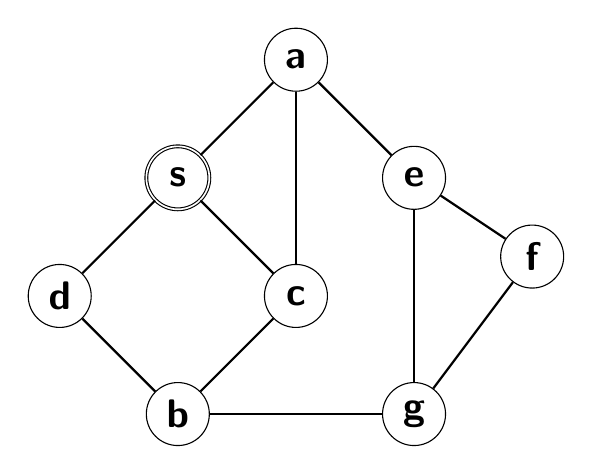
\begin{tikzpicture}[
    main_node/.style={circle, draw, font=\sffamily\Large\bfseries, minimum size=8mm},
    start_node/.style={circle, double, draw, font=\sffamily\Large\bfseries, minimum size=8mm}
]

% 定義節點位置 (Define node positions)
\node[main_node] (a) at (0, 3) {a};
\node[start_node] (s) at (-1.5, 1.5) {s};
\node[main_node] (e) at (1.5, 1.5) {e};
\node[main_node] (d) at (-3, 0) {d};
\node[main_node] (c) at (0, 0) {c};
\node[main_node] (f) at (3, 0.5) {f};
\node[main_node] (b) at (-1.5, -1.5) {b};
\node[main_node] (g) at (1.5, -1.5) {g};

% 連接節點 (Connect the nodes)
\path[draw, thick]
    (a) edge (s)
    (a) edge (c)
    (a) edge (e)
    (s) edge (d)
    (s) edge (c)
    (d) edge (b)
    (c) edge (b)
    (b) edge (g)
    (e) edge (f)
    (e) edge (g)
    (f) edge (g);

\end{tikzpicture}
\end{center}
s的dTime = 0\\
a的dTime =\underline{\hspace{2cm}}\\
b的dTime =\underline{\hspace{2cm}}\\
e的dTime =\underline{\hspace{2cm}}\\
f的dTime =\underline{\hspace{2cm}}
\end{graybox}

\begin{solution}
\textbf{详细分析:}

我们模拟广度优先搜索(BFS)的过程来确定每个顶点的发现时间(dTime)。dTime可以看作是顶点出队的顺序编号,从0开始。

\begin{table}[h!]
\centering
\begin{tabular}{|l|l|l|l|}
\hline
\textbf{步骤} & \textbf{出队顶点} & \textbf{dTime} & \textbf{队列状态 (队头 \(\to\) 队尾)} \\ \hline
0 (初始) & - & - & `[s]` \\ \hline
1 & \textbf{s} & \textbf{0} & `[a, c, d]` (s的邻居a,c,d按字母序入队) \\ \hline
2 & \textbf{a} & \textbf{1} & `[c, d, e]` (a的邻居c,e,s中,只有e未访问,入队) \\ \hline
3 & c & 2 & `[d, e, b]` (c的邻居a,b,s中,只有b未访问,入队) \\ \hline
4 & d & 3 & `[e, b]` (d的邻居b,s均已访问) \\ \hline
5 & \textbf{e} & \textbf{4} & `[b, f, g]` (e的邻居a,f,g中,f,g未访问,按序入队) \\ \hline
6 & \textbf{b} & \textbf{5} & `[f, g]` (b的邻居c,d,g均已访问) \\ \hline
7 & \textbf{f} & \textbf{6} & `[g]` (f的邻居e,g均已访问) \\ \hline
8 & g & 7 & `[]` (g的邻居b,e,f均已访问) \\ \hline
\end{tabular}
\end{table}

根据以上BFS过程:
\begin{itemize}
    \item 顶点 \textbf{a} 在第2步出队,其dTime为 \textbf{1}。
    \item 顶点 \textbf{e} 在第5步出队,其dTime为 \textbf{4}。
    \item 顶点 \textbf{b} 在第6步出队,其dTime为 \textbf{5}。
    \item 顶点 \textbf{f} 在第7步出队,其dTime为 \textbf{6}。
\end{itemize}

\hrulefill

s的dTime = 0\\
a的dTime =\underline{\hspace{2cm}\textbf{1}\hspace{2cm}}\\
b的dTime =\underline{\hspace{2cm}\textbf{5}\hspace{2cm}}\\
e的dTime =\underline{\hspace{2cm}\textbf{4}\hspace{2cm}}\\
f的dTime =\underline{\hspace{2cm}\textbf{6}\hspace{2cm}}
\end{solution}

\section*{168}
\begin{graybox}
从s开始,对以上无向图进行DFS,同一
顶点的邻居之间以a~z为序,求各顶点的
dTime和fTime
\begin{center}
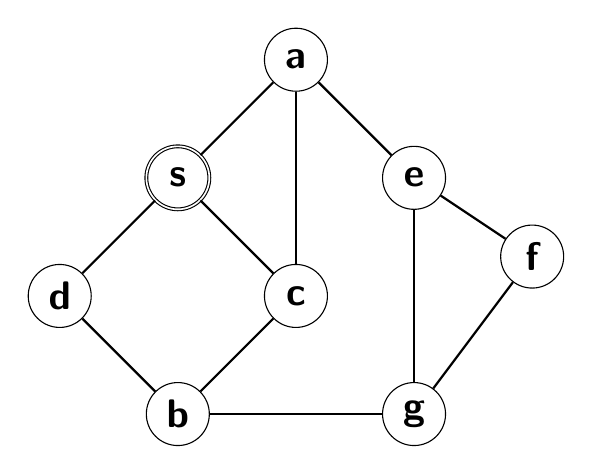
\begin{tikzpicture}[
    main_node/.style={circle, draw, font=\sffamily\Large\bfseries, minimum size=8mm},
    start_node/.style={circle, double, draw, font=\sffamily\Large\bfseries, minimum size=8mm}
]

% 定義節點位置 (Define node positions)
\node[main_node] (a) at (0, 3) {a};
\node[start_node] (s) at (-1.5, 1.5) {s};
\node[main_node] (e) at (1.5, 1.5) {e};
\node[main_node] (d) at (-3, 0) {d};
\node[main_node] (c) at (0, 0) {c};
\node[main_node] (f) at (3, 0.5) {f};
\node[main_node] (b) at (-1.5, -1.5) {b};
\node[main_node] (g) at (1.5, -1.5) {g};

% 連接節點 (Connect the nodes)
\path[draw, thick]
    (a) edge (s)
    (a) edge (c)
    (a) edge (e)
    (s) edge (d)
    (s) edge (c)
    (d) edge (b)
    (c) edge (b)
    (b) edge (g)
    (e) edge (f)
    (e) edge (g)
    (f) edge (g);

\end{tikzpicture}
\end{center}
s的dTime =0\\
s的fTime =15\\
c的dTime =\underline{\hspace{2cm}}\\
c的fTime =\underline{\hspace{2cm}}\\
g的dTime =\underline{\hspace{2cm}}\\
g的fTime =\underline{\hspace{2cm}}
\end{graybox}

\begin{solution}
\textbf{详细分析:}

我们通过模拟深度优先搜索(DFS)的递归过程来追踪每个顶点的发现时间(dTime)和完成时间(fTime)。一个全局计时器 `time` 从0开始。

\begin{enumerate}
    \item \textbf{DFS(s)}: `time=0`, `dTime(s)=0`, `time=1`. s的邻居(a,c,d).
    \item \textbf{DFS(a)}: `time=1`, `dTime(a)=1`, `time=2`. a的邻居(c,e,s).
    \item \textbf{DFS(c)}: `time=2`, `dTime(c)=2`, `time=3`. c的邻居(a,b,s).
    \item \textbf{DFS(b)}: `time=3`, `dTime(b)=3`, `time=4`. b的邻居(c,d,g).
    \item \textbf{DFS(d)}: `time=4`, `dTime(d)=4`, `time=5`. d的邻居(b,s)都已访问. \textbf{`fTime(d)=5`}, `time=6`. 返回b.
    \item 回到b. 邻居(c,d)已访问.
    \item \textbf{DFS(g)}: `time=6`, `dTime(g)=6`, `time=7`. g的邻居(b,e,f).
    \item \textbf{DFS(e)}: `time=7`, `dTime(e)=7`, `time=8`. e的邻居(a,f,g).
    \item \textbf{DFS(f)}: `time=8`, `dTime(f)=8`, `time=9`. f的邻居(e,g)都已访问. \textbf{`fTime(f)=9`}, `time=10`. 返回e.
    \item 回到e. 邻居(a,f,g)都已访问. \textbf{`fTime(e)=10`}, `time=11`. 返回g.
    \item 回到g. 邻居(b,e,f)都已访问. \textbf{`fTime(g)=11`}, `time=12`. 返回b.
    \item 回到b. 邻居(c,d,g)都已访问. \textbf{`fTime(b)=12`}, `time=13`. 返回c.
    \item 回到c. 邻居(a,b,s)都已访问. \textbf{`fTime(c)=13`}, `time=14`. 返回a.
    \item 回到a. 邻居(c,e,s)都已访问. \textbf{`fTime(a)=14`}, `time=15`. 返回s.
    \item 回到s. 邻居(a,c,d)都已访问. \textbf{`fTime(s)=15`}, `time=16`. 结束.
\end{enumerate}

\textbf{结果汇总:}
\begin{itemize}
    \item c: dTime = 2, fTime = 13
    \item g: dTime = 6, fTime = 11
\end{itemize}

\hrulefill

s的dTime =0\\
s的fTime =15\\
c的dTime =\underline{\hspace{2cm}\textbf{2}\hspace{2cm}}\\
c的fTime =\underline{\hspace{2cm}\textbf{13}\hspace{2cm}}\\
g的dTime =\underline{\hspace{2cm}\textbf{6}\hspace{2cm}}\\
g的fTime =\underline{\hspace{2cm}\textbf{11}\hspace{2cm}}
\end{solution}


\end{document}

% VScode 常用快捷键:

% Ctrl + R:                 打开最近的文件夹
% F2:                       变量重命名
% Ctrl + Enter:             行中换行
% Alt + up/down:            上下移行
% 鼠标中键 + 移动:           快速多光标
% Shift + Alt + up/down:    上下复制
% Ctrl + left/right:        左右跳单词
% Ctrl + Backspace/Delete:  左右删单词    
% Shift + Delete:           删除此行
% Ctrl + J:                 打开 VScode 下栏(输出栏)
% Ctrl + B:                 打开 VScode 左栏(目录栏)
% Ctrl + `:                 打开 VScode 终端栏
% Ctrl + 0:                 定位文件
% Ctrl + Tab:               切换已打开的文件(切标签)
% Ctrl + Shift + P:         打开全局命令(设置)

% Latex 常用快捷键

% Ctrl + Alt + J:           由代码定位到PDF
% 


% Git提交规范:
% update: Linear Algebra 2 notes
% add: Linear Algebra 2 notes
% import: Linear Algebra 2 notes
% delete: Linear Algebra 2 notes
